\section{Background}
\subsection{Neural Network}
\dmcmt{There was some general definitions of what an nn is in this section,
removed for now, nor really necessary, maybe can add a notation section if at
all necessary}

We conceptualize neural networks as directed acyclic graphs 
comprising three types of layers: the input layer, intermediate hidden layers, 
and the output layer. Our goal is to focus on the abstracting feed forward networks, 
where neuron values are computed based on preceding layer neuron values. 
Neurons in our network are denoted as $n_{(i,j)}$, where `$i$' signifies the 
neuron number in layer `$j$'. The weight matrix between layers `${j-1}$' and `$j$' 
is denoted as `$W_{{j-1}, j}$', and the bias matrix for layer `$i$' is denoted as 
`$B_{i}$'. The value of the `$i^{th}$' neuron in layer `$j$' is represented by 
`$v_{(i,j)}$', and `$V_{j}$' encompasses all such `$v_{(i,j)}$' values for layer 
`$j$'.

The computation of `$V_{j}$' involves applying an ``activation function ($\phi$)" 
to the ``weighted sum":

\[V_{j} = \phi(W_{{j-1}, j} \cdot V_{j-1} + B_{j}).\] 

We confine our activation function to the Rectified Linear Unit (ReLU), 
which can be expressed as $V_{j} = \max(W_{j-1, j} \cdot V_{j-1} + B_{j}, 0)$.


\begin{figure}[H]
    \centering
    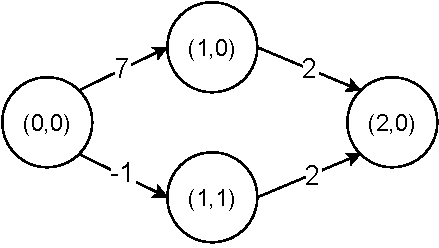
\includegraphics[width=0.3\textwidth, height = 0.15\textwidth]{diagrams/Basic_Neural_Network.pdf}
    \caption{A Simple Neural Network}
    \label{Figure: Simple Neurla}

\end{figure} 

Figure \ref{Figure: Simple Neurla} depicts a feed forward neural network 
comprising four neurons: $n_{(0, 0)}$, $n_{(1, 0)}$, $n_{(1, 1)}$, and $n_{(2, 0)}$. 
The weight matrix between layer 0 and layer 1, denoted by $W_{0,1}$, 
is $[7, -1]^T$, and the bias matrix for layer 1, denoted by $B_{1}$, 
is $[0, 0]^T$. If we assign a value of 1 to the neuron $n_{(0, 0)}$ 
(i.e., $v_{(0, 0)}=1$), then the value of the neuron $n_{(1,0)}$ is $v_{(1,0)}=7$, 
as determined by $V_{1} = \phi([7, -1]^{T} \cdot [1] + [0, 0]^{T}) = [7, 0]^{T}$.

\subsection{ Formal Analysis of Neural Networks }
\dmcmt{This section used to be titled Neural Network Verification, and explained
    the general idea of neural net verif, and some stuff on prop encoding. We
    are not doing exclusively verif. So, some more general and shorter
    discussion on formal analysis of nn added.}

Several techniques and methods have been studied to improve the reliability and
trustworthiness of \dnn deployed in safety critical settings via formal
analysis. This includes verifying \dnn with respect to a given
safety property \cite{reluplex, cegar-nn, deeppoly, cegarette, cleverest-nn,
conv-abs-gk, deep-abstract, lin-comb-abs-jan}, providing formal explanations of
the behavior of the \dnn \cite{minimal-image-fxai, overview-fxai}, and others.
\dmcmt{Is the and others okay? Ref the backdoor attacks work?} To provide the
formal guarantees behind the analysis performed, all of these techniques rely on
making \textit{neural network queries}. 

These neural network queries are of the form $(P, \mcnc, Q)$, and ask if
there is an input $x$ to $\mcnc$ for which the formula $P$ holds so that
the formula $Q$ holds on the output $\mcnc(x)$. While there are several
tools that can handle such queries, like \marabou and \abcrown, scalability
remains an issue, and so reducing the size of \cnc is desirable.

\subsection{Semantic Compressions and Abstractions with Empirical Guarantees}
\dmcmt{What is a better word than 'weak' here? Does 'empirical' work here?}

Several techniques utilise semantic information, typically extracted via
simulation of the \dnn, to obtain \abs. \dmcmt{Say: to improve scalability? }.
These can broadly be classified into two types. Neural network compression
techniques \todo{cite}, produce small \abs, but the behavior 
weaker guarantees.

\subsection{Neural Network Abstractions with Strong Guarantees}
\dmcmt{Do I need to contrast with Jan here? If so how much? 1 line? Yes, one
small section}

In this work, we focus on obtaining an abstract network \abs from a given
concrete network \cnc with formal guarantees linking the behavior of \abs and
\cnc so that formal analysis done on \abs can be lifted to \cnc. In particular,
we look for abstractions where $\forall x, \mabs(x) \geq \mcnc(x)$ \dmcmt{
Should I format this as definition?}. Since any
general neural network query can be converted to a query of the form $(P, \mcnc,
y > c)$ for some $c$ \cite{cegar-nn}, such an abstraction is extremely useful.
\dmcmt{Further explanation necessary?}

Furthermore, such guarantees are also useful for safe compression of \dnn.
Consider the case of medical diagnosis\todo{cite} or aircraft collisions, where
for safety reasons, a classifier should be biased towards not producing false
negatives. Guarantees such as above can formally ensure that the compressed \abs
never produces any more false negatives than \cnc. \todo{Ref next sections}.
\dmcmt{Should this be here?}

\subsection{Neural Network Splitting and Merging}

\dmcmt{Given that this section is critical to understanding our soundness
    guarantees, and that this is mostly existing work, how much space should be
spent here? Can we trust reader to read \cite{cegar-nn}}

\dmcmt{Start a running example here}

\dmcmt{Why Inc Dec? To get soundness. So, start by: to provide a strong formal
connection between \abs and \cnc, we follow the approach from
\cite{cegar-nn}. 2 diffs: 1. They focus on a safety prop, we aim to get
a general fw for any formal analysis not just safety verif. 2. We use inc-dec
only, not pos neg. That is sound because we can re-merge pos and neg versions
without changing behavior, since input weights are same, and max/min merge from
\cite{cegar-nn} doesn't depend on pos/neg.
Algos, diags unnecessary.
}

\dmcmt{Do we need to add a reference for 2-class?}

To transform \cnc into \abs so that the soundness guarantees hold, we follow
\cite{cegar-nn} to \textit{split} neurons in \cnc into copies labelled with
labels from \{\inc, \dec\} $\times$ \{\posc, \negc\} so that any
increase (decrease) in the value of a neuron labelled
\inc (\dec) only leads to an increase in output value. Then,
following \cite{cegar-nn}, a sound abstraction can be obtained by
\textit{merging} similarly labelled neurons as follows: if the neurons have the
label \inc (\dec), replace incoming edges from the same
previous layer neuron with a single edge with the maximum (minimum) of the
original edge weights. Outgoing edges to the same next layer neuron are replaced
with a single edge with the sum of the weights for both the \inc and \dec case.
\dmcmt{Is some notation necessary here? Its very clear to us, but could this be
    confusing for new readers? If so, should we spend space introducing notation
somewhere?}

We make a slight modification to the above: as a first optimization step, we
re-merge the two copies of the \abs neurons that are otherwise the same, but
have \posc and \negc labels respectively. This can always be done without
changing the behavior of the network since these copies will have the same \inc,
\dec labels and the same incoming weights. \dmcmt{Is this clear? Is it better to
write this as a lemma, and then put a proof in appendix?} This optimisation
allows us to discard the \posc and \negc class information, and reduces the size
of the maximally merged network.

\subsection{Refinement }
\dmcmt{This section should re-frame what gk's refinement does beyond cegar/verif
    into a more general fw. Then, it should point out the deficiencies (pulling
    out one neuron, singleton nodes, etc.) in this refinement approach and
    motivate the partial order. 
}

\dmcmt{    Do we talk about singleton nodes in intro or abstract? We were doing
    this in prev version. Also talk about refinement Jan, and briefly motivate
    what we would want to do.
}

\dmcmt{Not better, more controlled instead}

After merging the neurons, we introduce an over-approximation into 
the new network $\mathcal{N''}$. And since $\mathcal{N''}(x) \geq \mathcal{N}(x)$,
 there might exist a $x$, for which, $\exists x \in X, \hspace{1mm} \mathcal{N''}(x)
\geq c$ but $\nexists x \in X, \hspace{1mm} \mathcal{N}(x) \geq c$. 
Therefore, if a counter-example `$\beta$' returned is not a valid counter-example,
which means, $\mathcal{N''}(\beta) \geq c > \mathcal{N}(\beta)$, then, we must 
reverse some of the merges performed previously to get a new network which mitigates
the extent of the over-approximation for us to get a valid counter-example or to 
prove that the original property is valid.

In \cite{cegar-nn}, the authors employed a Counterexample-Guided Abstraction 
Refinement (CEGAR) approach to eliminate the spurious counter-examples. 
They utilized a counter-example ($\beta$) to identify a neuron $n_{(i, j)}$ 
that had been merged into the node `$r$' for refinement. The authors then 
computed the value $\omega$ which was equal to 
$|v_i^j(\beta) - r(\beta)| \cdot |w_{n_{(i-1, k)},n_{(i,j)}}-w_{n_{i-1,k},r}|$, 
where $v_{(i, j)}(\beta)$ denotes the value of $n_{(i, j)}$ at the 
counter-example $\beta$, $r(\beta)$ denotes the value of the 
representative neuron $r$ at the counter-example $\beta$, $w_{n_{(i-1,k)},n_{(i,j)}}$ 
denotes the weight between a neuron $n_{i-1,k}$ and a neuron $n_{i,j}$. 
If this value $\omega$ was over a recommended amount $\epsilon$, they proceeded to 
separate $n_{(i, j)}$ from $r$ to potentially eliminate the spurious counter-example 
$\beta$.

\dmcmt{ 
    An example of Elboher's Refinement where we get a lot of singletons
}


 In the next section, we present a new method for merging neurons in 
 order to reduce the number of refinement steps, thereby expediting the 
 verification process.
